% --------------------------------------------------
% 
% This chapter is for dingo
% 
% --------------------------------------------------

% DEFINITIONS
\def\RR{{\mathbb R}}

% COMMANDS
\newcommand{\dd}[1]{\mathrm{d}#1}
\newcommand{\OO}{\mathcal{O}\xspace}
\newcommand{\sO}{\widetilde{\mathcal{O}}\xspace}

% To make lem work
\newtheorem{thm}{Theorem}
\newtheorem{lem}[thm]{Lemma}


\chapter{Software development to establish metabolic flux sampling 
         approaches at the community level}
\label{cha:dingo}


\section{A New MCMC Algorithm for Sampling the Flux Space of
Metabolic Networks}

\textbf{Citation:} Chalkis, A., Fisikopoulos, V., Tsigaridas E. and Zafeiropoulos H.\\ 
Geometric Algorithms for Sampling the Flux Space of Metabolic Networks. \\ 
37th International Symposium on Computational Geometry (SoCG 2021) \\ 
DOI: \href{10.4230/LIPIcs.SoCG.2021.21}{10.4230/LIPIcs.SoCG.2021.21} 

\subsection{Abstract}
\label{sec:mmcs-abstract}

   Systems Biology is a fundamental field and paradigm that introduces a new era in Biology.
   The crux of its functionality and usefulness relies on metabolic networks
   that model the reactions occurring inside an organism
   and provide the means to understand the underlying mechanisms that govern biological systems.
   Even more, metabolic networks have a broader impact that ranges from
   resolution of ecosystems to personalized medicine.

   The analysis of metabolic networks is a computational geometry oriented field
   as one of the main operations they depend on is sampling uniformly points from  polytopes;
   the latter provides a representation of the steady states of the metabolic networks.
   However, the polytopes that result from biological data are of very high dimension (to the order of thousands) and in most, if not all, the cases are considerably skinny.
   Therefore, to perform uniform random sampling efficiently in this setting, we need
   a novel algorithmic and computational framework specially tailored
   for the properties of metabolic networks.

   We present a complete software framework to handle sampling in metabolic networks.
   Its backbone is a Multiphase Monte Carlo Sampling (MMCS) algorithm
   that unifies rounding and sampling in one pass, obtaining both upon termination.
   It exploits an
   improved variant of the Billiard Walk that enjoys faster arithmetic complexity per step.
   We demonstrate the efficiency of our approach by performing extensive experiments
   on various metabolic networks.
   Notably, sampling on the most complicated human metabolic network accessible today, Recon3D,
   corresponding to a polytope of dimension  $5\,335$, took less than $30$ hours.
   To our knowledge, that is out of reach for existing software.





\subsection{Introduction}
\label{sec:mmcs-intro}

   \subsubsection*{The field of Systems Biology}

   Systems Biology establishes a scientific approach and a paradigm. As a
   research approach, it is the qualitative and quantitative study of the systemic
   properties of a biological entity along with their ever evolving interactions
   \cite{klipp2016systems, kohl2010systems}.
   By combining experimental studies  with mathematical
   modeling it analyzes the function and the behavior of biological systems.
   In this setting, we model the interactions between the  components of a system
   to shed light  on the system's \textit{raison d'être} and to decipher its underlying mechanisms
   in terms of evolution, development, and physiology \cite{ideker2001new}.

   Initially, Systems Biology emerged as a need. New technologies in Biology
   accumulate vast amounts of information/data from different levels of the
   biological organization, i.e., genome, transcriptome, proteome, metabolome
   \cite{quinn2016sample}. This leads to the emerging question \textit{"what shall
   we do with all these pieces of information"?} The answer, if we consider
   Systems Biology as a paradigm, is to move away from reductionism, still the main
   conceptual approach in biological research, and adopt holistic approaches for
   interpreting how a system's properties emerge~\cite{noble2008music}. The
   following diagram provides a first, rough, mathematical formalization of this
   approach.

   \begin{center}
   \textit{components} $\,\to\,$ \textit{networks} $\,\to\,$ \textit{in silico models} $\,\to\,$\textit{phenotype} \cite{palsson2015systems}. \\ \end{center}

   %  Metabolism
   Systems Biology expands in all the different levels of living entities, from the
   molecular, to the organismal and ecological level. The notion that
   penetrates all  levels horizontally is \emph{metabolism}; the
   process that modifies molecules and  maintains the living state of a
   cell or an organism through a set of chemical reactions
   \cite{schramski2015metabolic}. The reactions begin with a particular molecule
   which they convert into some other molecule(s), while they are catalyzed by
   enzymes in a key-lock relationship.
   We call the quantitative relationships between the components of a reaction   \emph{stoichiometry}.
   Linked reactions, where the product of the first acts as the substrate for the
   next, build up metabolic pathways. Each pathway is responsible for a certain
   function. We can link together the aggregation of all the pathways that take
   place in an organism (and their corresponding reactions)
   and represent them mathematically using  the reactions' stoichiometry.
   Therefore, at the species level, metabolism is a network of its metabolic pathways and we call
   these representations \emph{metabolic networks}.


   \subsubsection*{From metabolism to computational geometry}

   The complete reconstruction of the metabolic network of an organism is a
   challenging, time consuming, and computationally intensive task; especially for species of high level of complexity such as \emph{Homo sapiens}.
   Even though sequencing the complete genome of a species is becoming a trivial task
   providing us with quality insight, manual curation is still mandatory and large groups 
   of researchers need to spend a great amount of time to build such models \cite{thiele2010protocol}.
   However, over the last few years, automatic reconstruction approaches for building genome-scale metabolic 
   models \cite{machado2018fast} of relatively high quality have been developed.
   Either way, we can now obtain the metabolic network of a bacterial species (single cell species)
   of a tissue and even the complete metabolic network of a mammal.
   Biologists are also moving towards obtaining such networks for all the species present in a microbial community. This will allow us to further investigate the dynamics, the functional profile, and the inter-species reactions that occur.
   Using the stoichiometry of each reaction, which is always the same in the various species,
   we convert the metabolic network of an organism to a mathematical model.
   Thus, the metabolic network becomes an \emph{in silico} model of the knowledge it represents.
   
   % Definitions and background
   In metabolic networks analysis mass and energy are considered to be conserved
   \cite{palsson2009metabolic}. As many homeostatic states, that is steady internal
   conditions \cite{shishvan2018homeostatic}, are close to steady states (where the
   production rate of each metabolite equals its consumption rate
   \cite{cakmak2012new}) we commonly use the latter in metabolic networks analysis.

   Stoichiometric coefficients are the number of molecules a biochemical reaction
   consumes and produces. The coefficients of all the reactions in a network,
   with $m$ metabolites and $n$ reactions ($m < n$),  form
   the \emph{stoichiometric matrix} $S\in \RR^{m\times n}$~\cite{palsson2015systems}.
   %
   % The flux space
   The nullspace of $S$ corresponds to the steady states of the network:
   \begin{equation}
   \label{eq:Sv}
   S \cdot x = 0 ,
   \end{equation}
   where $x \in \RR^n $ is the \textit{flux vector} that contains  the fluxes
   of each chemical reaction of the network.
   %
   Flux is the rate of turnover of molecules through a metabolic pathway.
   % Methodology
   \begin{figure}[!htbp]
      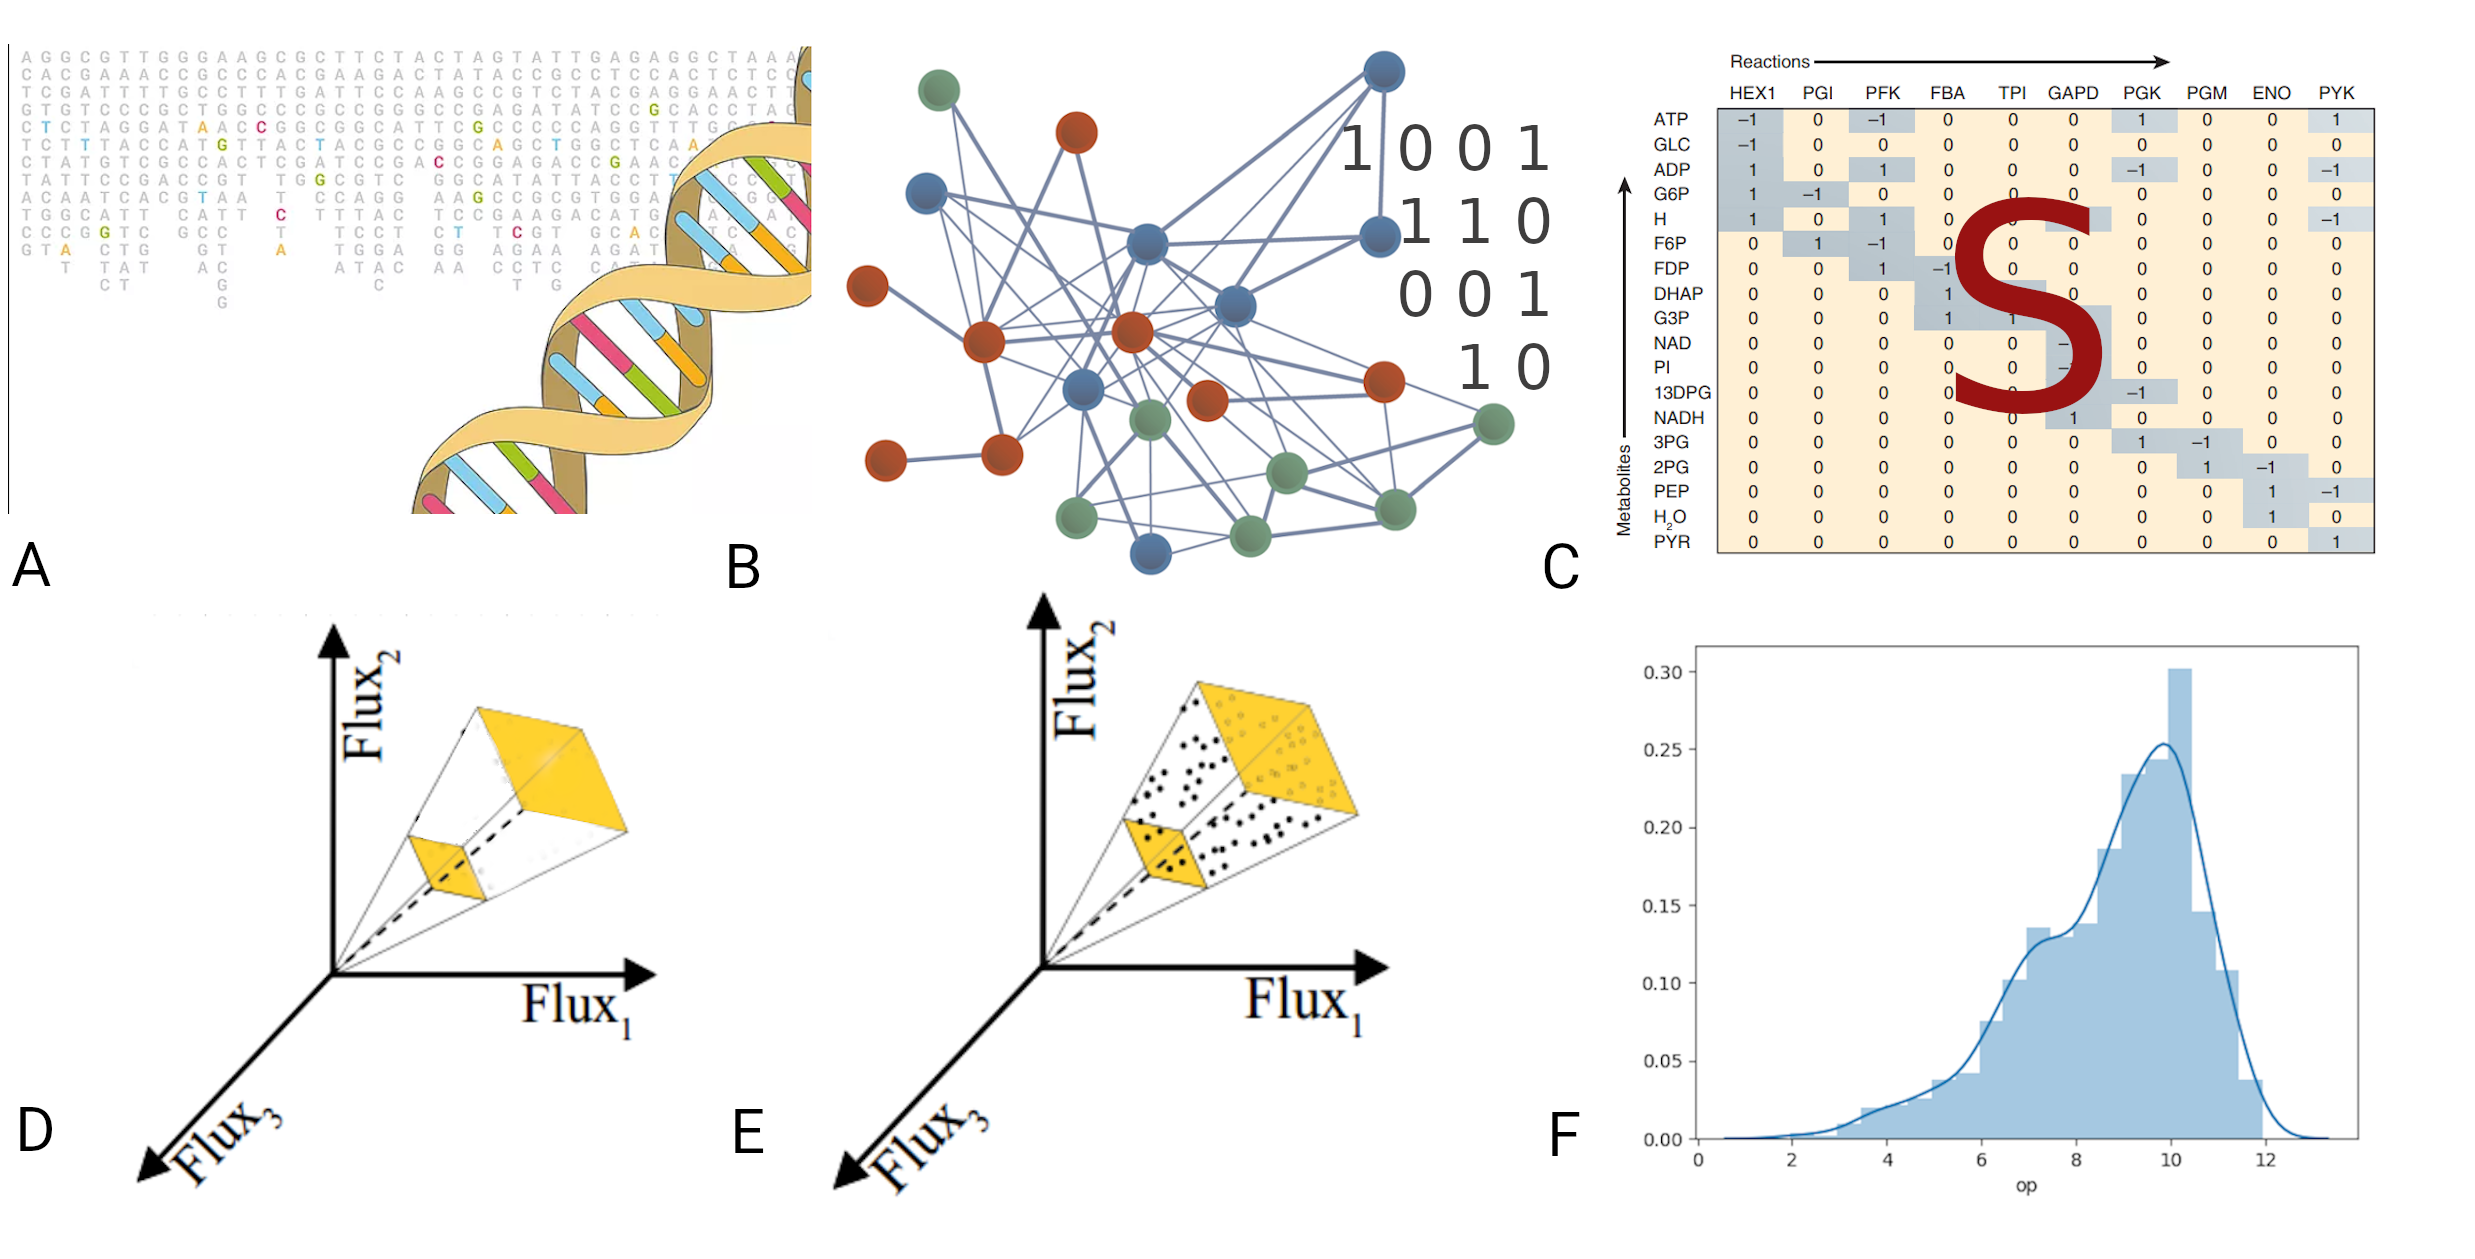
\includegraphics[width=1.0\columnwidth]{figures/flux_sampling_workflow.png}
      \caption[From DNA sequences to distributions of metabolic fluxes]{
         From DNA sequences to distributions of metabolic fluxes.
         (A) The genes of an organism provide us with the enzymes that it can potentially produce. Enzymes are like a blueprint for the reactions they can catalyze.
         (B) Using the enzymes we identify the reactions in the organism.
         (C) We construct the stoichiometric matrix of the metabolic  model.
         (D) We consider the flux space under different conditions (e.g., steady states);
         they correspond  to  polytopes containing flux vectors addressing these conditions.
         (E) We sample from polytopes that are typically skinny and of high dimension.
         (F) The distribution of the flux of a reaction provides  great insights
         to biologists.
      }
      \label{fig:sampling_workflow}
   \end{figure}

   % But why being interested in such a task ? The genome of most bacteria are rather short to have issues like that. 
   % However, MAGs can be brought together and build the metabolic model of a whole community! 

   All physical variables are finite, therefore  the flux (and the concentration)
   is bounded  \cite{palsson2015systems}; that is
   for each coordinate $x_i$ of the $x$, there are $2n$ constants
   $x_{ub, i}$ and  $x_{lb, i}$
   such that  $x_{lb,i} \le x_i \le x_{ub, i}$, for $i  \in [n]$.
   We derive the constraints from explicit experimental information.
   In cases where there is no such information, reactions are left unconstrained by
   setting arbitrary large values to their corresponding bounds according to their reversibility properties; i.e., if a reaction is reversible then its flux might be negative as well~\cite{lularevic2019improving}.
   The constraints define a $n$-dimensional box
   containing both the steady and the dynamic states of the system.
   If we intersect that box with the nullspace of
   $S$, then we define a polytope that encodes all the possible steady
   states and their  flux distributions \cite{palsson2015systems}.
   We call it the  steady-state \emph{flux space}.
   Fig.~\ref{fig:workflow} illustrates the complete workflow from building a metabolic network to the computation of a flux distribution.
   
   % FBA & limitations
   Using the polytopal representation, a commonly used method for the analysis of a metabolic network is Flux Balance Analysis (FBA)~\cite{orth2010flux}.
   FBA identifies a single optimal flux distribution by optimizing a linear objective function over a polytope~\cite{orth2010flux}. Unfortunately, this is a \textit{biased} method because it depends on the  selection of the objective function.
   %%
   To study the  global features of a metabolic network we need \emph{unbiased methods}. To obtain  an accurate picture of the whole solution space we exploit sampling techniques \cite{schellenberger2009use}.
   If collect a sufficient number of points uniformly distributed in the interior of the polytope, then the biologists can study the properties of certain components of the whole network and deduce significant biological insights~\cite{palsson2015systems}. Therefore, efficient sampling tools are of great importance.
   
   % COPULAS ON RECOND 3D
   \begin{figure}[h]
      \centering
      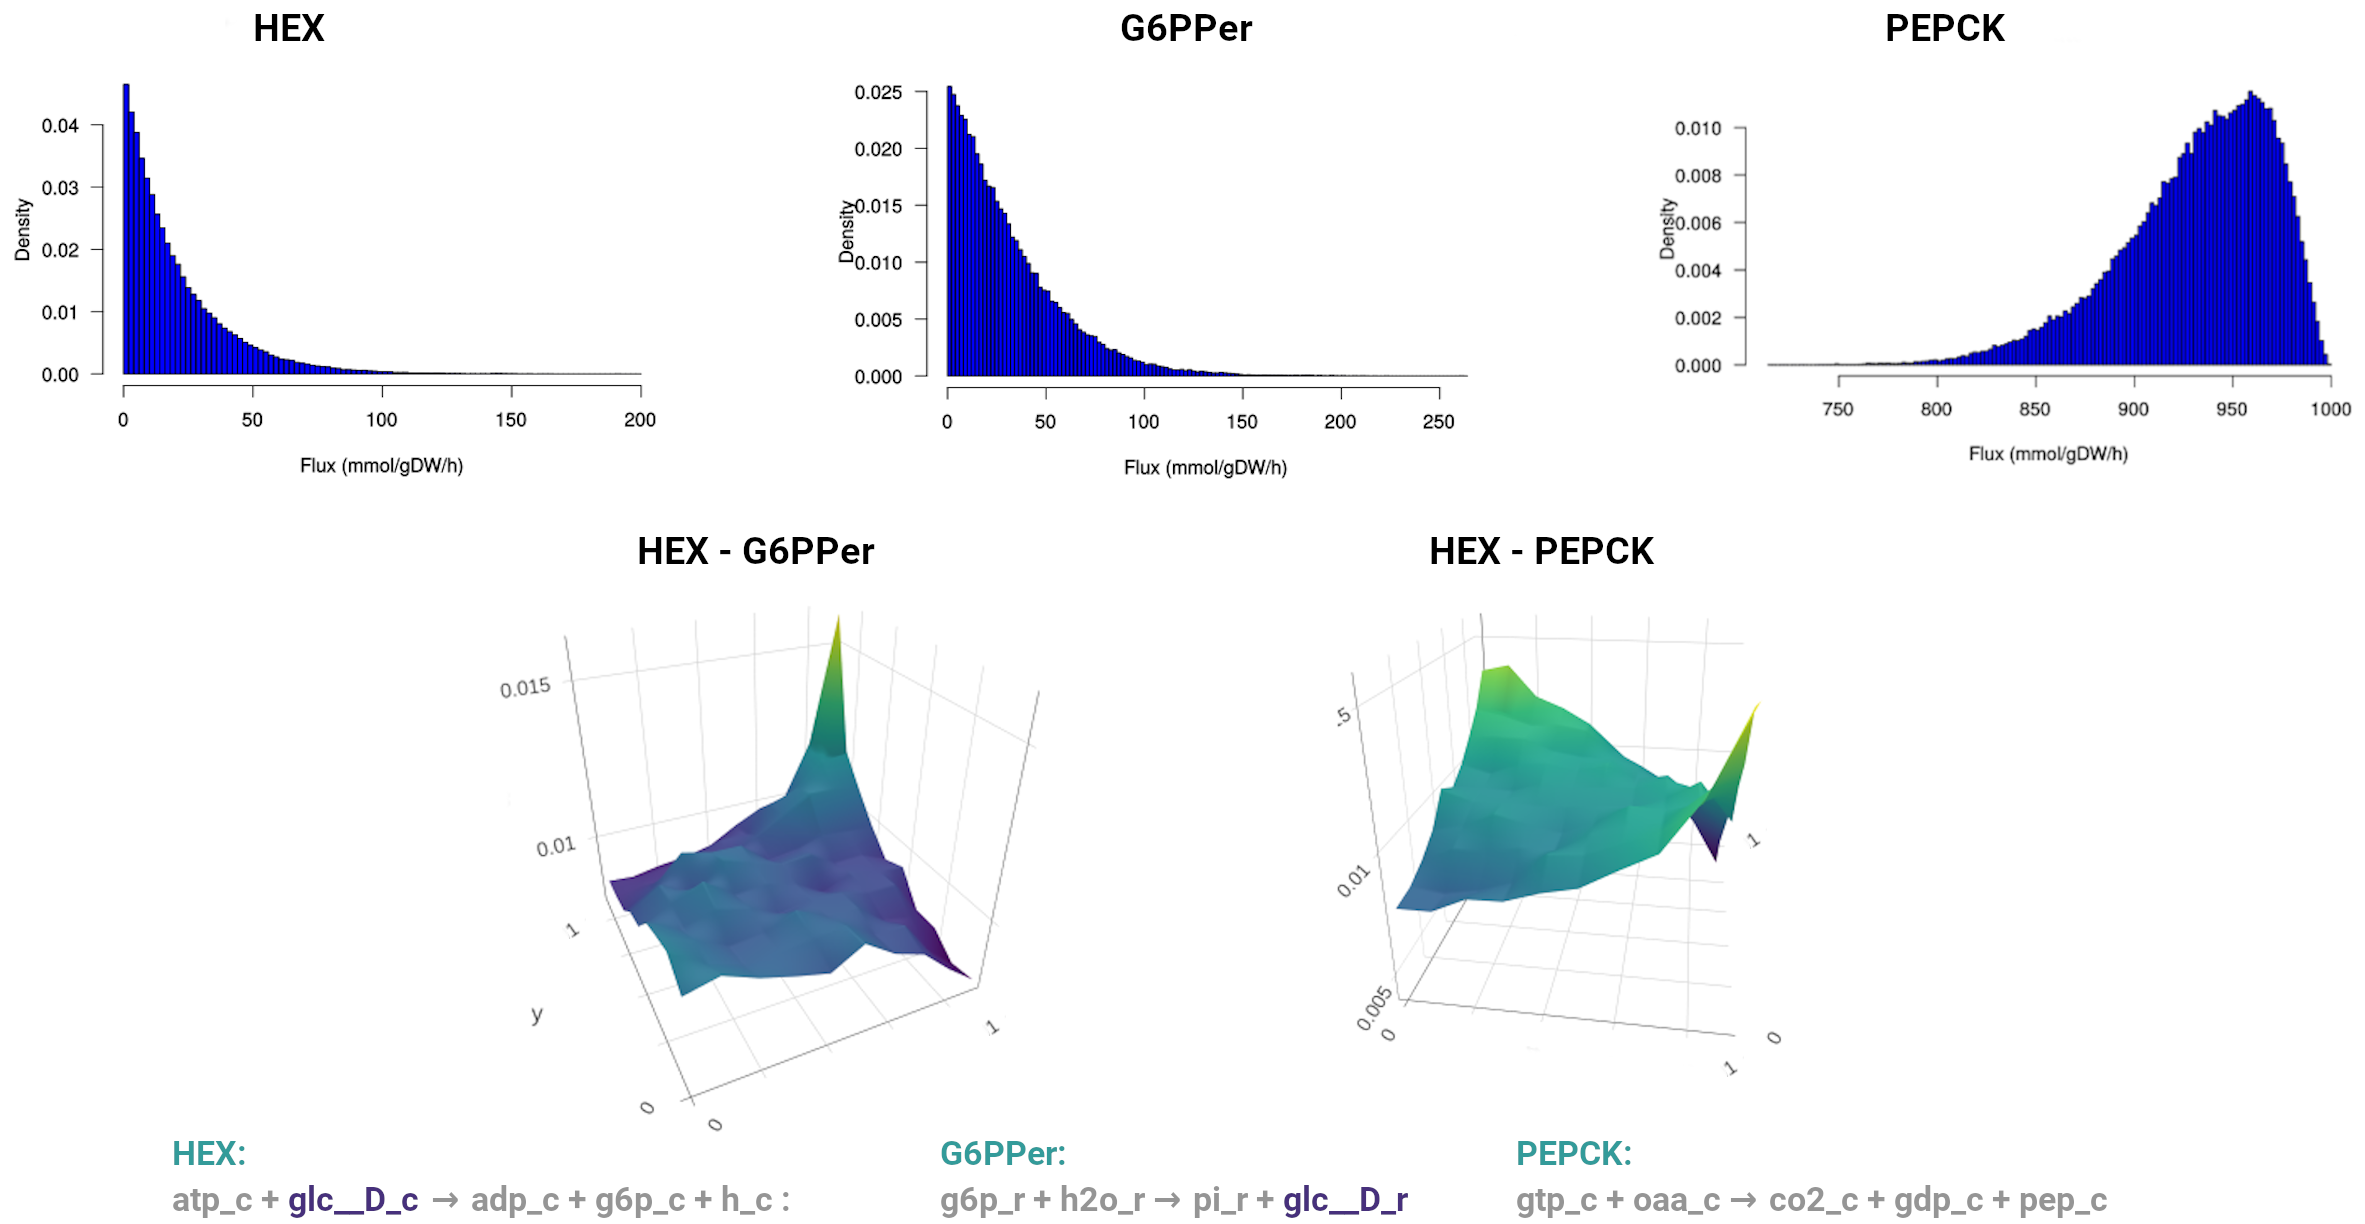
\includegraphics[width=125mm]{figures/copulas_cropped.png}
      \caption[Flux distributions in the most recent human metabolic network Recon3D]{
         Flux distributions in the most recent human metabolic network Recon3D~\cite{brunk2018recon3d}. 
         We estimate the flux distributions of the reactions catalyzed by the enzymes Hexokinase (D-Glucose:ATP) (HEX), Glucose-6-Phosphate Phosphatase, Edoplasmic Reticular (G6PPer)
         and Phosphoenolpyruvate carboxykinase (GTP) (PEPCK).
         As we sample steady states, the production rate of $glc\_\_D \_c$ should be equal to its consumption rate. 
         Thus, in the corresponding copula, we see a positive dependency between HEX,
         i.e., the reaction that consumes $glc\_\_D \_c$ and G6PPer, that produces it.
         Furthermore, the PEPCK reaction operates when there is no $glc\_\_D\_c$ available and does not operate when the latter is present.
         Thus, in their copula we observe a negative dependency between HEX and PEPCK.
         A copula is a bivariate probability distribution for which the marginal probability distribution of each variable is uniform.
         It implies a positive dependency when the mass of the distribution concentrates along the up-diagonal (HEX - G6PPer)
         and a negative dependency when the mass is concentrated along the down-diagonal (HEX - PEPCK). %~\cite{Cales18}.
         The bottom line contains the  reactions and their stoichiometry.
      }
      \label{fig:copulas}
   \end{figure}


   \subsubsection*{Metabolic networks through the lens of random sampling} 
   \label{subsec:previous_work}

   Efficient uniform random sampling on polytopes resulting from metabolic
   networks is a very challenging task  both from the theoretical (algorithmic)
   and the engineering (implementation)  point of view.
   % computational geometry and the computer science point of view.
   First, the dimension of the polytopes is of the order of certain thousands. This
   requires, for example, advanced engineering techniques to cope with memory
   requirements and to perform linear algebra operations with large matrices;
   e.g., in
   Recon3D~\cite{brunk2018recon3d} we compute the null space of a
   $8\,399 \times 13\,543$ matrix. Second, the polytopes are rather skinny
   (Sec.~\ref{sec:experiments}); this makes it harder for sampling algorithms to
   move in the interior of polytopes and calls for novel practical techniques to
   sample.

   There is extended on-going research concerning advanced algorithms and
   implementations for sampling metabolic networks over the last decades. Markov
   Chain Monte Carlo algorithms such as Hit-and-Run (HR)~\cite{smith84} have been
   widely used to address the challenges of sampling. Two variants of HR are the
   non-Markovian Artificial Centering Hit-and-Run
   (ACHR)~\cite{kaufman1998direction} that has been widely used in sampling
   metabolic models, e.g.,~\cite{Saa16}, and Coordinate Hit-and-Run with Rounding
   (CHRR)~\cite{haraldsdottir2017chrr}. 
   The latter is part of the \texttt{cobra} toolbox~\cite{heirendt2019creation}, the most commonly used software package for the analysis of metabolic networks. 
   CHRR enables sampling from complex metabolic
   networks corresponding to the highest dimensional polytopes so far. There are
   also stochastic formulations where the inclusion of experimental noise in the
   model makes it more compatible with the stochastic nature of biological
   networks~\cite{MacGillivray17}. The recent study in~\cite{fallahi2020comparison}
   offers an overview as well as an experimental comparison of the currently
   available samplers.

   These implementations played a crucial role in actually performing in practice
   uniform sampling from the flux space. However, they are currently limited to
   handle polytopes of dimension say $\leq 2\, 500$ \cite{fallahi2020comparison,
   haraldsdottir2017chrr}. This is also the order of magnitude of the most
   complicated, so far, metabolic network model built,
   Recon3D~\cite{brunk2018recon3d}. By including $13\,543$ metabolic reactions and
   involving $4 \,140$ unique metabolites, Recon3D provides a representation of the
   $17\%$ of the functionally of annotated human genes. To our knowledge, there is
   no method that can efficiently handle sampling from the flux space of Recon3D.

   Apparently, the dimension of the polytopes will keep rising and not only for the ones corresponding to  human metabolic networks.
   %issue highlight important as integrated methods for improved human metabolic models will provide great assistant in precision medicine applications.
   % where drug responses can be assessed in the context of individual patient-specific genomes.
   Metabolism governs systems biology at all its levels, including the one of the community.
   Thus, we are not only interested in sampling a sole metabolic network, even if it has the challenges of the human.
   Sampling in polytopes associated to network of networks are the next big thing in metabolic networks analysis and in Systems Biology \cite{bernstein2019metabolic,perez2016metabolic}.

   Regarding the sampling process, from the theoretical point of view, we are
   interested in the convergence time, or \textit{mixing time}, of the Markov Chain,
   or geometric \textit{random walk}, to the target distribution. Given a
   $d$-dimensional polytope $P$, the mixing time of several geometric random walks
   (e.g., HR or Ball Walk) grows quadratically with respect to the sandwiching
   ratio $R/r$ of the polytope~\cite{LovSim,Lovasz06}. Here $r$ and $R$ are the
   radii of the smallest and largest ball with center the origin that contains, and
   is contained, in $P$, respectively; i.e., $rB_d \subseteq P \subseteq RB_d$,
   where $B_d$ is the unit ball. It is crucial to reduce $R/r$, i.e., to put $P$ in
   well a rounded position where 
   $R/r = \sO(\sqrt{d})$; 
   the $\sO(\cdot)$ notation
   means that we are ignoring polylogarithmic factors. A powerful approach to
   obtain well roundness is to put $P$ in \emph{near isotropic position}. In
   general, $K \subset \RR^d$ is in isotropic position if the uniform distribution
   over $K$ is in isotropic position, that is $\mathbb{E}_{X\sim K}[X] = 0$ and
   $\mathbb{E}_{X\sim K}[X^TX] = I_d$, where $I_d$ is the $d\times d$ identity
   matrix. Thus, to put a polytope $P$ into isotropic position one has to generate
   a set of uniform points in its interior and apply to $P$ the transformation that
   maps the point-set to isotropic position; then iterate this procedure until $P$
   is in $c$-isotropic position \cite{ Cousins15,Lovasz06}, for a constant~$c$.
   In~\cite{Adamczak10} they prove that $\OO(d)$ points suffice to achieve
   $2$-isotropic position. Alternatively in \cite{haraldsdottir2017chrr} they
   compute the maximum volume ellipsoid in $P$, they map it to the unit ball, and
   then apply to $P$ the same transformation. They experimentally show that a few
   iterations suffice to put $P$ in John's position~\cite{John48}. Moreover, there
   are a few algorithmic contributions that combine sampling with distribution
   isotropization steps, e.g., the multi-point walk~\cite{Bertsimas04} and the
   annealing schedule~\cite{Kalai06}.

   An important parameter of a random walk is the \textit{}{walk length}, i.e., the number of the intermediate points that a random walk visits before producing a single sample point.
   The longer the walk length of a random walk is, the smaller the distance of the current distribution to the stationary (target) distribution becomes.
   For the majority of  random walks there are bounds on the walk length to bound the mixing time with respect to a statistical distance. For example, HR generates a sample from a distribution with total variation distance less than $\epsilon$ from the target distribution after $\sO(d^3)$~\cite{Lovasz06} steps, in a well rounded convex body and for log-concave distributions. Similarly, CDHR mixes after a polynomial, in the diameter and the dimension, number of steps~\cite{Laddha20,Narayanan20} for the case of uniform distribution. However, extended practical results have shown that both CDHR and HR converges after $\OO(d^2)$ steps~\cite{Chalkis19, Cousins15, haraldsdottir2017chrr}. The leading algorithms for uniform polytope sampling are the Riemannian Hamiltonian Monte Carlo sampler~\cite{VempalaRiem18} and the Vaidya walk~\cite{Chen18}, with mixing
   times $\sO(md^{2/3})$ and $\sO(m^{1/2}d^{3/2})$ steps, respectively.
   However, it is not clear if these random walks can outperform CDHR in practice,
   because of their  high cost per step and numerical instability.

   Billiard Walk (BW)~\cite{Gryazina14} is a random walk that employs linear
   trajectories in a convex body with boundary reflections; alas with an unknown
   mixing time. The closest guarantees for its mixing time are those of HR and
   stochastic billiards~\cite{Dieker15}. Interestingly,~\cite{Gryazina14} shows
   that, experimentally, BW converges faster than HR for a proper tuning of its
   parameters. The same conclusion follows from the computation of the volume of
   zonotopes~\cite{Chalkis20}. It is not known how the sandwiching ratio of $P$
   affects the mixing time of BW. Since BW employs reflections on the boundary,
   we can consider it as a special case of Reflective Hamiltonian Monte Carlo~\cite{ChePioCaz18}.


   For almost all random walks the theoretical bounds on their mixing times are
   pessimistic and unrealistic for  computations. Hence,
   if we terminate the random walk earlier, we generate samples that are  usually highly correlated.
   There are several \textit{MCMC Convergence Diagnostics} \cite{Roy20} to check
   if  the quality of a  sample can  provide an accurate
   approximation of the target distribution. For a dependent sample, a powerful
   diagnostic is the \textit {Effective Sample Size} (ESS). It is the number of
   effectively independent draws from the target distribution that the Markov chain
   is equivalent to. For autocorrelated samples, ESS bounds
   the uncertainty in estimates \cite{geyer92} and provides  information about
   the quality of the sample. There are several statistical tests to evaluate the quality of a generated sample, e.g., potential scale reduction factor (PSRF)~\cite{Gelman92}, maximum mean discrepancy (MMD)~\cite{Gretton12},
   %(two-sample test)
   and the uniform tests~\cite{CousinsThesis17}.
   %%
   Interestingly, 
   the copula representation we employ in Fig.~\ref{fig:copulas} to capture the dependence between two fluxes of reactions was also used  successfully in a geometric framework to detect financial crises capturing the dependence between portfolio return and volatility~\cite{Cales18}.

   % MMCS CONTRIBUTION
\subsection{Contribution}
\label{sec:mmcs-contribution}


   We introduce a Multi-phase Monte Carlo Sampling (MMCS) algorithm
   (Sec.~\ref{sec:MMCS} and Alg.~\ref{alg:MMCS}) to sample from a polytope~$P$. In
   particular, we split the sampling procedure in phases where, starting from $P$,
   each phase uses the sample to round the polytope. This improves the efficiency
   of the random walk in the next phase, see Fig.~\ref{fig:mmcs_phases}.
   For sampling, we propose an improved variant of Billiard Walk (BW)
   (Sec.~\ref{subsec:billiard} that enjoys faster
   arithmetic complexity per step. We also handle efficiently the potential arithmetic inaccuracies near to the boundary, see~\cite{ChePioCaz18}.
   %
   We accompany the MMCS algorithm with a powerful MCMC diagnostic, namely the
   estimation of Effective Sample Size (ESS), to identify a satisfactory
   convergence to the uniform distribution.
   However, our method is flexible and  we can
   use any  random walk and
   combination of MCMC diagnostics to decide~
   convergence.

   The open-source implementation of our algorithms\footnote{\url{https://github.com/GeomScale/volume_approximation/tree/socg21}} provides a
   complete software framework to handle efficiently sampling in metabolic
   networks. We demonstrate the efficiency of our tools by performing experiments
   on almost all the metabolic networks that are publicly available and by
   comparing with the
   state-of-the-art software packages as \textit{cobra}
   (Sec.~\ref{subsec:experiments}). Our implementation is faster than \textit{cobra}
   for low dimensional models,  with a speed-up that ranges from $10$ to $100$ times;
   this gap on running times increases for bigger models
   (Table~\ref{tab:results1}). The quality of the sample our software produces is
   measured with two widely used diagnostics, i.e., ESS and potential scale reduction factor (PSRF)~\cite{Gelman92}. The highlight of
   our method is the ability to sample from the most complicated human metabolic
   network that is accessible today, namely Recon3D. In Fig.~\ref{fig:copulas} we estimate marginal univariate and bivariate flux distributions in Recon3D which validate
   (a) the  quality of the sample by confirming a mutually exclusive pair of biochemical pathways,
   and that (b) our method indeed generates steady states. In particular, our software
   can sample $1.44\cdot 10^5$ points from a $5\,335$-dimensional polytope in a day
   using modest hardware. This set of points suffices for the majority of systems
   biology analytics.
   To our understanding this task is out of reach for existing software.
   Last, MMCS algorithm is quite general sampling scheme and
   so it has the potential to address other
   hard computational problems like  multivariate integration and volume estimation of polytopes.


   % --------------  like a "bridge" ------------

   % In the next section we present a thorough description of both the biological and the geometrical
   % notions that are the backbone of our framework. 
   % Section~\ref{sec:billiard}
   % details the Billard Walk random walk, while we introduce our Multiphase Monte Carlo
   % Sampling algorithms in 
   % Section~\ref{sec:MMCS}.
   % Finally, in
   % Section~\ref{sec:experiments} 
   % we present our open-source implementation and various
   % experimental results to highlight he potential our approach. 
   % We conclude in
   % Section~\ref{sec:conclusion}, where we also present some future directions.




% MMCS METHODS
\subsection{Methods \& Implementation}
\label{sec:mmcs-methods}

\subsubsection*{Efficient Billiard walk}
\label{subsec:mmcs-methods-bw}

   The geometric random walk of our choice
   to sample from a polytope
   is based on  Billiard Walk (BW)~\cite{Gryazina14},
   which we modify to reduce the per-step cost.

   For a polytope $P = \{ x \in \RR^d \,|\, A x \leq b  \}$,
   where $A \in \RR^{k \times d}$ and $b \in \RR^k$,
   BW starts from a given point $p_0 \in P$,
   selects uniformly at random a
   direction, say $v_0$, and it moves along the direction of $v_0$ for length $L$;
   it reflects on the boundary if necessary. This results a new point $p_1$ inside
   $P$. We repeat the procedure from $p_1$. Asymptotically it converges to the
   uniform distribution over $P$. The length is $L=-\tau \ln \eta$, where $\eta$ is
   a uniform number in $(0,1)$, that is $\eta\sim\mathcal{U}(0,1)$, and $\tau$ is a
   predefined constant. It is useful to set a bound, say $\rho$, on the number of
   reflections to avoid computationally hard cases where the trajectory may stuck
   in corners. In \cite{Gryazina14} they set
   $\tau \approx \mathop{diam}(P)$ and $\rho =10d$.
   Our choices for $\tau$ and $\rho$ depend on a
   burn-in step that we detail in  Sec.~\ref{sec:experiments}.

   At each step of BW we
   compute the intersection point of a ray, say $\ell:=\{p+tv,\ t\in\RR_+ \}$,
   with the boundary of $P$, $\partial P$, and the normal vector of the tangent
   plane at the intersection point.
   The inner vector of the facet that the intersection  point belongs to is a row of $A$.
   To compute the point $\partial P\cap\ell$ where the first reflection of a BW
   step takes place, we solve the following $m$ linear equations
   \begin{equation}\label{eq:boundary_oracle}
   a_j^T(p_0 + t_jv_0) = b_j \Rightarrow t_j = (b_j - a_j^Tp_0) / a_j^Tv_0,\ j \in[k],
   \end{equation}
   and keep the smallest positive $t_j$; $a_j$ is the $j$-th row of the matrix $A$.
   We solve each equation in $\OO(d)$ operations
   and so the overall complexity is $\OO(dk)$.
   A straightforward approach for BW would consider that each reflection costs $\OO(kd)$ and thus the per step cost is $\OO(\rho kd)$.
   However, our improved version performs more efficiently both \textit{point} and \textit{direction updates} by storing computations from the previous iteration combined with a preprocessing step. The preprocessing step involves the normal vectors of the facets, that takes $m^2 d$ operations,
   and the amortized per-step complexity of BW becomes $\OO((\rho + d)k)$.

   \begin{lem}
   \label{lem:BW-step-cost}
   The amortized per step complexity of BW is $\OO((\rho + d)k)$ after a preprocessing step that takes $\OO(k^2d)$ operations, where $\rho$ is the maximum number of reflections per step.
   \end{lem}

   % proof
   \begin{proof}
      The first reflection of a Billiard Walk step costs $O(kd)$.
      During its computation, we store all the values of the inner
      products $a_j^Tx_0$ and $a_j^Tu_0$.
      At the reflection $i>0$, we start from a point $x_i$
      and the solutions of the corresponding linear equations are
      \label{eq:billiard_implementation1}
      \begin{equation*}
      \begin{split}
         \cr a_j^T(p_i + t_ju_i) = b_j & \Rightarrow \\
         \cr a_j^T(p_{i-1} + t_{i-1}u_{i-1})
         + t_ja_j^T(u_{i-1}-2(u_{i-1}^Ta_r) a_r) = b_j  & \Rightarrow \\
         \cr t_j = \frac{b_j - a_j^T(p_{i-1} +  t_{i-1}u_{i-1})}{a_j^T(u_{i-1}-2(u_{i-1}^Ta_r) a_r)},\
         \text{ for }  j \in [k]  ,
         \end{split}
      \end{equation*}

      \begin{equation}\label{eq:billiard_implementation2}
      \text{ and } \, u_{i+1} = u_i -2(u_i^Ta_l) a_l,
      \end{equation}
      where $a_r,\ a_l$ are the normal vectors of the facets that $\ell$ hits at reflection $i-1$ and $i$ respectively, and $t_{i-1}$ the solution of the  reflection $i-1$.
      The index $l$ of the normal $a_l$
      corresponds to the equation with the smallest positive $t_j$
      in~(\ref{eq:billiard_implementation1}).
      We solve each of the  equations in (\ref{eq:billiard_implementation2}) in $O(1)$ based on our bookkeeping from the  previous reflection.
      We also store the inner product $u_i^Ta_l$ in (\ref{eq:billiard_implementation2}) from the  previous reflection.
      After computing all $a_i^Ta_j$ as a preprocessing step, which takes $k^2d$ operations, the total per-step cost of Billiard Walk is $O((d+\rho)k)$.
   \end{proof}




   The use of floating point arithmetic could result to points outside $P$ due to rounding errors when computing boundary points. To avoid this, when we compute the roots in Equation~(\ref{eq:boundary_oracle}) we exclude the facet that the ray hit in the previous reflection.


   % BW ALGO - alg:billiard
   \begin{figure}[!htp]
      \centering
      \textbf{Algorithm 1: }Billiard Walk$(P, p, \rho, \tau, W)$
      \medskip
      \label{alg:billiard}

      \begin{algorithmic}
         \REQUIRE polytope $P$; point $p \in P$; upper bound on the number of reflections
         $\rho$; \\ parameter $\tau$ to adjust the length of the trajectory; walk length $W$.
         \ENSURE a point in $P$ (uniformly distributed in $P$).
         \FOR {$j=1,\dots ,W$} 
         \STATE {
            $L \leftarrow -\tau\ln\eta$;  $\ \eta\sim \mathcal{U}(0,1) \quad$ \COMMENT{\textit{length of the trajectory}}
            $i\leftarrow 0 \quad $ \COMMENT{\textit{current number of reflections}}
            $p_0\leftarrow p \quad $ \COMMENT{\textit{initial point of the step}}
            pick a uniform vector $u_0$ from the unit sphere
            \COMMENT{\textit{initial direction}}
         }
         \WHILE{$i\leq \rho$}
         \STATE{$\ell \leftarrow \{p_i + tu_i, 0\leq t\leq L\} \quad$} \COMMENT{\textit{this is a segment}}

         \IF{$\partial P\cap\ell=O$} 
            \STATE{$p_{i+1} \leftarrow p_i+Lu_i \quad$
                  \textbf{break} \;}
         \ENDIF
         
         \STATE{$p_{i+1} \leftarrow \partial P\cap\ell ; \quad$}
         \COMMENT{\textit{point update}}
            
         \STATE{the inner vector, $s$, of the tangent plane at $p$, \\
            \ \ s.t.\ $||s|| = 1$,\; $L \leftarrow L - |P\cap\ell|$,
         $u_{i+1} \leftarrow u_i - 2(u_i^Ts) s \quad$}
         \COMMENT{\textit{direction update}}

         \STATE{$i \leftarrow i+1$}

         \ENDWHILE
      
         \IF{$i=\rho$}
            \STATE{$p \leftarrow p_0$}
         \ELSE	
            \STATE{$p \leftarrow p_i$}
         \ENDIF
         

         \ENDFOR

      \RETURN $p$\;


      \end{algorithmic}
         
   \end{figure}

   At each step of Billiard Walk, we compute the intersection point of a ray, say
   $\ell:=\{p+tu,\ t\in\mathbb{R}_+ \}$,
   with the boundary of $P$, $\partial P$, and the normal vector of the tangent
   plane of $P$ at the intersection point.
   The inner vector of the facet that the intersection  point belongs to is a row of $A$.
   To compute the point $\partial P\cap\ell$ where the first reflection of a Billiard Walk
   step takes place we need to compute the intersection of $\ell$ with all the hyperplanes that define the facets of $P$.
   This corresponds to solve (independently) the following $m$ linear equations
   \begin{equation}
     a_j^T(p_0 + t_ju_0) = b_j \Rightarrow t_j = (b_j - a_j^Tp_0) / a_j^Tu_0,\ j \in[k],
   \end{equation}
   and keep the smallest positive $t_j$; $a_j$ is the $j$-th row of the matrix $A$.
   We solve each equation in $\mathcal{O}(d)$ operations and so the overall complexity is
   $\mathcal{O}(d k)$, where $k$ is the number of rows of $A$ and thus an upper bound on
   the number of facets of $P$. A straightforward approach for Billiard Walk would
   consider that each reflection costs $\mathcal{O}(k d)$ and thus the per step cost is
   $\mathcal{O}(\rho kd)$. However, our improved version performs more efficiently both
   \textit{point} and \textit{direction updates} in pseudo-code by storing some
   computations from the previous iteration combined with a preprocessing step. The
   preprocessing step involves the normal vectors of the facets and takes $k^2 d$
   operations. So the amortized per-step complexity of Billiard Walk becomes
   $\mathcal{O}((\rho + d)k)$. The pseudo-code appear in Algorithm~\ref{alg:billiard}.
   
   
   
   % lemma 
   % \begin{lem}
   %     \label{lem:BW-step-cost}
   %     The amortized cost per step complexity of Billiard Walk
   %     (Algorithm~\ref{alg:billiard}) is $O((\rho + d)k)$ 
   %     after a preprocessing step that takes $O(k^2d)$ operations, where $\rho$ is the maximum number of reflections per step.
   %  \end{lem}



   \subsubsection*{Multiphase Monte Carlo Sampling algorithm}
   \label{subsec:mmcs-methods-algor}


   To sample steady states in the flux space of a metabolic network, with $m$
   metabolites and $n$ reactions, we introduce a Multiphase Monte Carlo Sampling
   (MMCS) algorithm; it is multiphase because it consists of a sequence of sampling
   phases.

   Let $S\in\mathbb{R}^{m\times n}$ be the  stoichiometric matrix
   and  $x_{lb},\ x_{ub}\in\mathbb{R}^{n}$
   bounds on the fluxes.
   The flux space is the bounded convex polytope

   \begin{equation}
   \label{eq:steady_states}
      \mathrm{FS} :=  \{x \in \RR^n \,|\, Sx = 0,\ x_{lb}\leq x \leq x_{ub} \} \subset \RR^n .
   \end{equation}

   The dimension, $d$, of $\mathrm{FS}$ is smaller than the dimension of the
   ambient space; that is $d \leq n$.
   %%
   To work with a full dimensional polytope we restrict the box
   induced by the inequalities $x_{lb}\leq x \leq x_{ub}$ to the null space of  $S$.
   Let the  H-representation of the box be
   $\left\{ x \in \RR^n \,\Big |\, \begin{pmatrix} I_n \\ -I_n\end{pmatrix} x
   \leq \begin{pmatrix} x_{ub} \\ x_{lb} \end{pmatrix} \right\}$,
   where $I_n$ is the $n\times n$ identity matrix,
   and let $N\in\RR^{n\times d}$ be the matrix of the null space of $S$,
   that is $S \, N = 0_{m \times d}$.
   Then
   $P = \{ x\in\RR^d\ |\ A x \leq b \}$,
   where $A = \begin{pmatrix} I_n N \\ -I_n N\end{pmatrix}$
   and $b = \begin{pmatrix} x_{ub} \\ x_{lb} \end{pmatrix}  N$,
   is a
   full dimensional polytope (in $\RR^d$).
   After we sample (uniformly) points from $P$,
   we transform them to uniformly distributed points (that is steady states) in $\mathrm{FS}$
   by applying  the linear map induced by $N$.
   %%

   \vspace{8pt}
   MMCS generates, in a sequence of sampling phases, a set of points,
   that is almost equivalent to $n$ independent uniformly distributed points in $P$, where $n$ is given.
   %%
   At each phase, it employs Billiard Walk (Section~\ref{subsec:billiard}) 
   to sample approximate uniformly distributed points, rounding
   to speedup sampling,
   and uses the Effective Sample Size (ESS) diagnostic to decide termination.
   The pseudo-code of the algorithm appears in Alg.~\ref{alg:MMCS}.


   \emph{Overview.} Initially we set $P_0 = P$.

   At each phase $i \geq 0$ we sample at most $\lambda$ points from $P_i$. We
   generate them in chunks; we also call them  \emph{chain} of sampling points.
   Each chain contains at  most $l$ points (for simplicity consider $l = \OO(1)$). To
   generate the points in each chain we employ BW, starting from a point inside
   $P_i$; the starting point is different for each chain.
   We repeat this procedure until the total number of samples in $P_i$ reaches the maximum number $\lambda$; we need $\tfrac{\lambda}{l}$ chains.
   To compute a starting point for a chain, we pick a point uniformly at random in the
   Chebychev ball of $P_i$ and we perform $\OO(\sqrt{d})$
   burn-in BW steps to obtain a warm start.

   After we have generated  $\lambda$ sample points we perform
   a rounding step on $P_i$ to obtain the polytope of the next phase, $P_{i+1}$.
   %%
   We compute a linear transformation, $T_i$, that puts the sample
   into isotropic position and then $P_{i+1} = T_i(P_i)$.
   The efficiency of BW improves from one phase to the next one
   because the sandwiching ratio decreases and so
   the  average number of reflections decreases
   and thus the convergence  to the uniform distribution accelerates
   (Section~\ref{subsec:experiments}).
   That is we obtain faster a sample of better quality.
   Finally, the (product of the) inverse transformations maps the samples to $P_0 = P$. Fig.~\ref{fig:mmcs_phases}
   depicts the procedure.


   \emph{Termination.} There are no bounds on the mixing time of BW \cite{Gryazina14},
   hence for termination we rely on ESS.
   MMCS terminates when the minimum ESS among all the univariate
   marginals is larger than a requested value. We chose the marginal
   distributions (of each flux) because they are essential for systems biologists,
   see \cite{Bordel10} for a typical example.
   In particular, after we generate a chain, the algorithm updates the ESS of each
   univariate marginal to take into account all the points that we have sampled in $P_i$,
   including the newly generated chain. We keep the minimum, say $n_i$, among all
   marginal ESS values. If $\sum_{j=0}^in_j$ becomes larger than $n$ before the
   total number of samples in $P_i$ reaches the upper bound $\lambda$, then  MMCS
   terminates. Otherwise, we proceed to the next phase. In summary, MMCS terminates
   when the sum of the minimum marginal ESS values of each phase reaches $n$.


   % THE MMCS PHASES
   \begin{figure}[!htbp]
      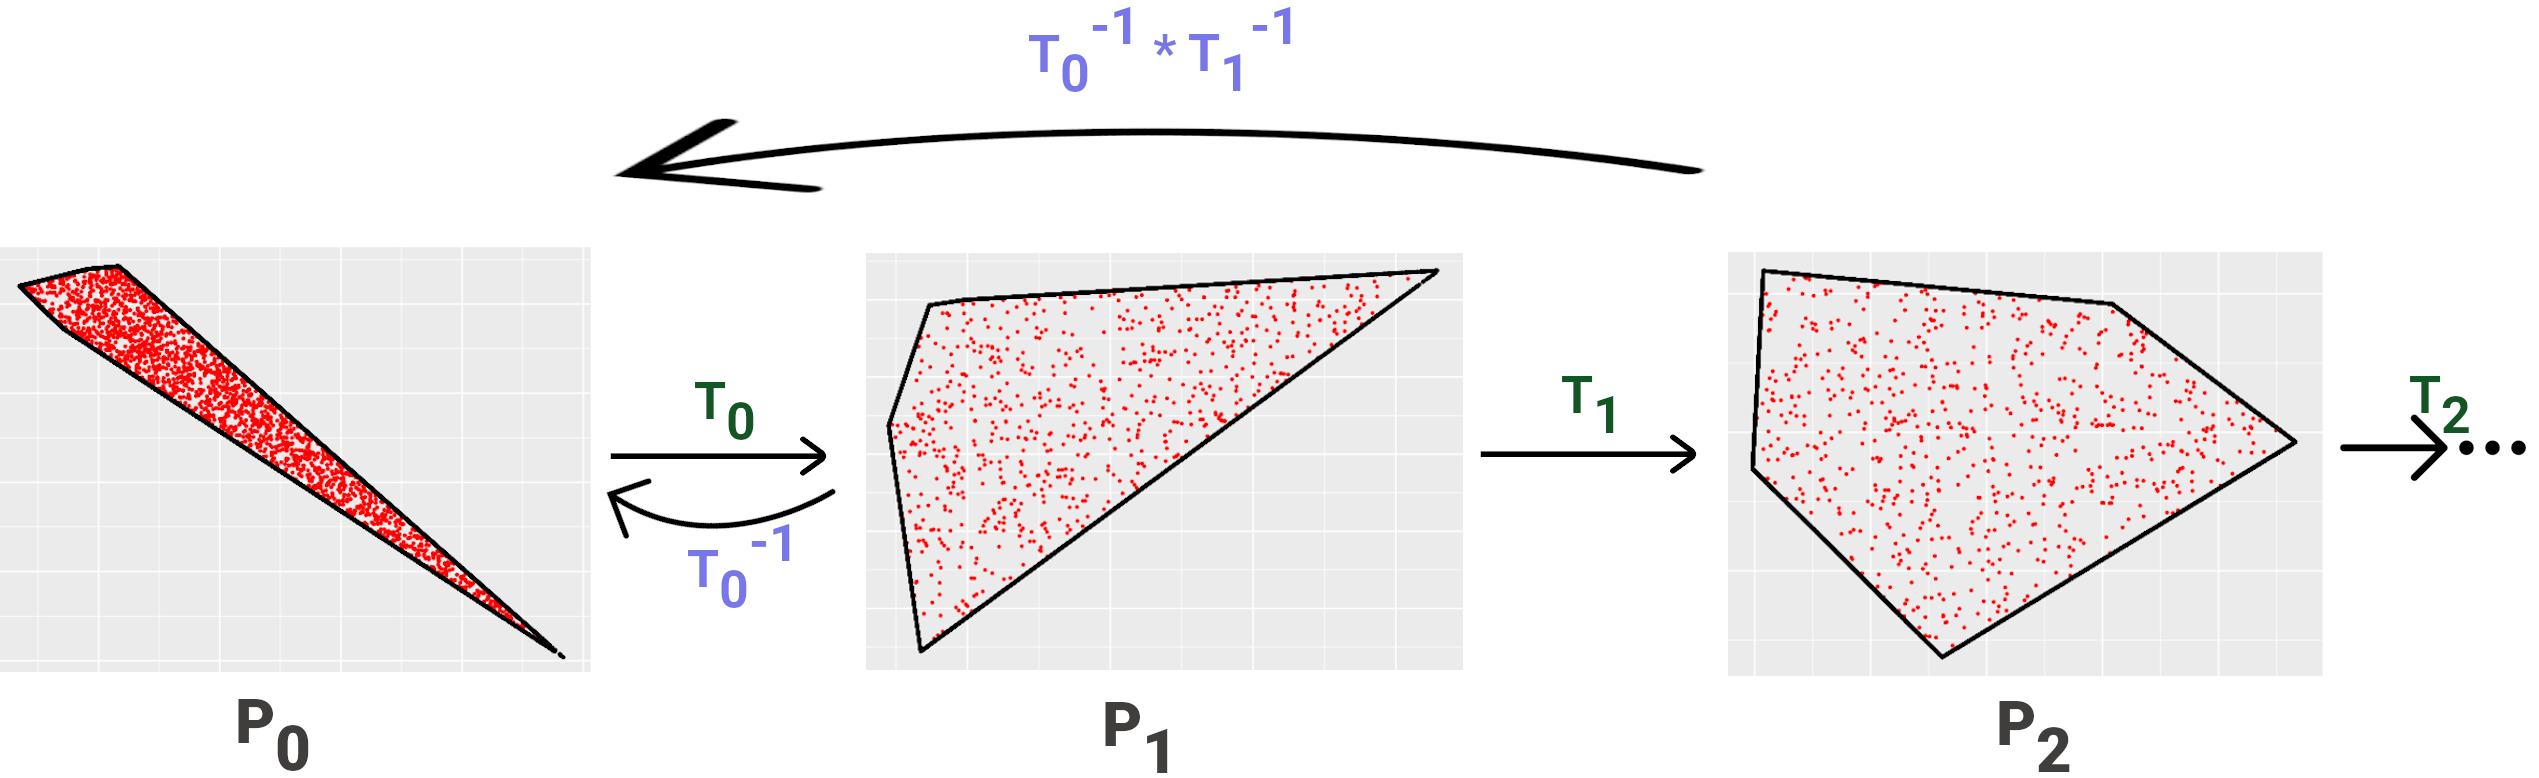
\includegraphics[width=1.0\columnwidth]{figures/sampling_extra_phase_croped.png}
      \caption[A Multiphase Monte Carlo Sampling algorithm]{
         An illustration of our Multiphase Monte Carlo Sampling algorithm. The method is given an integer $n$ and starts at phase $i=0$ sampling from $P_0$. In each phase it samples a maximum number of points $\lambda$. If the sum of Effective Sample Size in each phase becomes larger than $n$ before the total number of samples in $P_i$ reaches $\lambda$ then the algorithm terminates. Otherwise, we proceed to a  new phase.
    We map back to $P_0$ all the generated samples of each phase.
      }
      \label{fig:mmcs}
   \end{figure}




   % MMCS ALGO 2
   \begin{figure}
      \label{alg:MMCS}
      \centering
      \textbf{Algorithm 2:} Multiphase \\ Monte Carlo Sampling$(P, n, l, \lambda, \rho, \tau, W)$
      \medskip
      \begin{algorithmic}

      \REQUIRE
      A full dimensional polytope $P\in\mathbb{R}^d$; \\
      requested effectiveness $n\in\mathbb{N}$ (number of sampled points); \\
      $l$ length of each chain;\\ $\lambda$ upper bound of the number of generated points in each phase $\lambda$;  \\
      upper bound on the number of reflections $\rho$;\\
      parameter $\tau$ to adjust the length of the  trajectory; walk length $W$.

      \item[]
      
      \ENSURE
      a set $n$ of approximate uniformly distributed points $S\in P$

      \item[]

      \STATE{Set $P_0 \leftarrow P,\ sum\_ess\leftarrow 0,\ S\leftarrow\emptyset,\ i\leftarrow 0,\ T_0 = I_d$}

      \WHILE{$sum\_ess < n$}

         \STATE{$sum\_point\_phase\leftarrow 0,\ U\leftarrow\emptyset$}
      
         \WHILE{$sum\_point\_phase < \lambda$;}
         
            \STATE{Set $Q \leftarrow \emptyset$; Generate a starting point $q_0\in P_i$; }

            \FOR{$j=1,\dots ,l$}
               \STATE{$q_j \leftarrow$Billiard\_Walk($P_i, q_{j-1}, \rho, \tau, W$),\;
               Store the point $q_j$ to the set $Q$ \
            }
            \ENDFOR
            

            $S\leftarrow S\cup T_i^{-1}(Q)$,\;
            $U\leftarrow U\cup Q$,\;
            $sum\_point\_phase\leftarrow sum\_point\_phase + l$\;
            Update ESS $n_i$ of this phase\;
            %$k\leftarrow n_i$\;
            \IF{$sum\_ess + n_i \geq n$} 
            \STATE{
               \textbf{break}
            }
            \ENDIF

         \ENDWHILE

         \STATE{$sum\_ess\leftarrow sum\_ess + n_i$,\;  
         Compute $T$ such that $T(U)$ is in isotropic position,\;
         $P_{i+1} \leftarrow T(P_i)$,\;
         $T_{i+1} \leftarrow T_i\circ T$,\;
         $i\leftarrow i+1$
         }
         
      \ENDWHILE
   
      \RETURN $S$
      \end{algorithmic}
   \end{figure}



   \emph{Rounding step}. This step is
   motivated by the theoretical result in~\cite{Adamczak10} and the rounding
   algorithms~\cite{Lovasz06, Cousins15}.
   We apply the linear transformation $T_i$ to $P_i$
   so that the sandwiching ratio of $P_{i+1}$ is smaller than that of $P_i$.
   %This also improves (progressively) the efficiency of BW (Sec.~\ref{sec:experiments}).
   To find the suitable $T_i$ we compute  the SVD decomposition of the matrix that contains the sample row-wise \cite{Shiri20}.
   
   \emph{Updating the  Effective Sample Size.}
   %%
   The effective sample size of a sample of points generated by a process with autocorrelations $\rho_t$ at lag $t$
   is function (actually an infinite series) in the $\rho_t$'s; its exact value is unknown.
   Following \cite{geyer92}, we efficiently compute ESS employing a finite sum of monotone estimators
   $\hat{\rho}_t$ of the autocorrelation at lag $t$, by exploiting Fast Fourier Transform. 
   Furthermore, given $M$ chains of samples, the autocorrelation estimator $\hat{\rho}_t$ is given by,
   $\hat{\rho}_t = 1 - \frac{C - \frac{1}{M}\sum_{i=1}^{M}\hat{\rho}_{t,i}}{B}$, 
   where $C$ and $B$ are the within-sample variance estimate and the multi-chain variance estimate given in \cite{Gelman92} and $\hat{\rho}_{t,i}$ is an estimator of the autocorrelation of the $i$-th chain at lag $t$.
   To update the ESS, for every new chain of points the algorithm generates, we compute
   $\hat{\rho}_{t,i}$. Then, using Welford's algorithm we
   update the average of the estimators of autocorrelation at lag $t$,
   as well as the between-chain variance and the within-sample variance estimators given in~\cite{Gelman92}.
   Finally, we update the ESS using these estimators.
   
   
   \begin{lem}\label{lem:mmcs_complexity}
   Let $P=\{x\in\RR^d\ |\ Ax\leq b\}$, $A\in\RR^{k\times d},\ b\in\RR^k$ a full dimensional polytope in $\RR^d$.
   The total number of operations per phase that Alg.~\ref{alg:MMCS} performs, is
   $\OO(W(\rho + d)k\lambda + \lambda^2d + d^3)$,
   where $W$ is the walk length for Billiard Walk.
   \end{lem}
   

   To update the ESS, for every new chain of points the algorithm generates, we compute
   the estimator of its autocorrelation. Then, using Welford's algorithm we
   update the average of the estimators of autocorrelation at lag $t$,
   as well as the between-chain variance and the within-sample variance estimators~\cite{Gelman92}.
   Finally, we update the ESS using these estimators.
   
   
   \begin{lem}[Complexity of MMCS per phase]
     \label{lem:mmcs_complexity}
     Let $P=\{x\in\mathbb{R}^d\ |\ Ax\leq b\}$, where $A\in\mathbb{R}^{k\times d}$ and
     $b\in\mathbb{R}^k$, be a full dimensional polytope in $\mathbb{R}^d$.
     %%
     To sample $n$ points  (approximately) uniformly distributed in $P$,
     MMCS (Algorithm~\ref{alg:MMCS}) performs
     $\mathcal{O}(W(\rho + d)k\lambda + \lambda^2d + d^3)$
     arithmetic operations per phase, where $W$ is the walk length
     of Billiard Walk,
     $\rho$ is an upper bound on the number of reflections, and $\lambda$
     and upper bound on the points generated at each phase.
   \end{lem}
   
   % Cost per step of BW
   \begin{proof}
       The cost per step of Billiard Walk is $O((\rho + d)k)$. In each phase we
       generate, using Billiard Walk, at most $\lambda$ points with walk length $W$.
       Thus, the cost to generate these points is $O(W(\rho + d)k\lambda)$.
     
        To compute the starting point of each chain the algorithm picks a random point
        uniformly distributed in the Chebychev ball of $P$ and performs $\mathcal{O}(1)$
        Billiard Walk steps starting from it.
        The former  takes $\mathcal{O}(d)$ operations and the latter  takes $\mathcal{O}(W(\rho + d)k)$ operations.
        The total number of chains is $\mathcal{O}(\lambda / l) = \mathcal{O}(\lambda)$, as $l=\mathcal{O}(1)$.
        Thus, the total cost to generate all the starting points is $\mathcal{O}(d\lambda + W(\rho + d)k\lambda)$. The update of ESS for each univariate marginal requires $\mathcal{O}(1)$ operations, since $l = \mathcal{O}(1)$.
     
        If the termination criterion has not been met after generating $\lambda$ points,
        then
        the algorithm computes a linear transformation to put the set of points to isotropic
        position. We do this by computing the SVD decomposition of the matrix that
        contains the set of points row-wise. This corresponds to an SVD of a
        $\lambda \times d$ matrix and takes $O(\lambda^2d + d^3)$ operations
        \cite{golub13}.
   \end{proof}

   In Section~\ref{sec:experiments} we discuss how to tune the parameters of MMCS
   to make it more efficient in practice. We also comment on the (practical)
   complexity of each phase, based on the tuning.





% MMCS RESULTS
\subsection{Results}

% MMCS DISCUSSION
\subsection{Discussion}

   Flux sampling at the community level!












   
% From \citet{price2004genome} :
% "Pairwise correlation coefficients can be calculated
% between all reaction fluxes based on uniform random
% sampling. Perfectly correlated reactions (R2 = 1) operate
% as functional modules within a biochemical network,
% whereas uncorrelated reactions (R2 ~0) operate independently of each other. The degree of independence
% between reactions is an important consideration when
% choosing a set of fluxes to measure that will best determine the operating state of a biochemical network"


% Write something from \citeauthor{polanyi1968life}

% \section{The `dingo` Python library}






